\documentclass{beamer}

% Theme of presentation
\mode<presentation>
{
	\usetheme{Madrid}
	\usecolortheme{orchid}
}

% Information about presentation
\title{Sample presentation}
\subtitle{in \LaTeX\ Beamer}
\institute{Nazarbayev University}
\author{Adilet Zhaxybay}

% Uncomment this, if you want the table of contents to pop up at
% the beginning of each section/subsection:
\AtBeginSection[]
{
  \begin{frame}<beamer>{Outline}
   \tableofcontents[currentsection,currentsubsection]
  \end{frame}
}
\AtBeginSubsection[]
{
  \begin{frame}<beamer>{Outline}
    \tableofcontents[currentsection,currentsubsection]
  \end{frame}
}

\begin{document}

% Title slide
\begin{frame}
	\titlepage
\end{frame}

% Slide with outline
\begin{frame}{Table of contents}
  \tableofcontents
\end{frame}

\begin{frame}{Introduction}
	\begin{block}{\LaTeX\ Beamer}
		LaTeX Beamer is a powerful tool to create presentations
	\end{block}
	\pause
	\begin{block}{Export to PDF}
		It produces platform-independent presentations in PDF
	\end{block}	
\end{frame}

\section{Slides with text}

\begin{frame}{Blocks}
	\begin{block}{This is block}
		Using \textit{blocks} is a handy way to present your text
	\end{block}
	\pause
	\begin{block}{Pause between}
		You can also insert a pause between blocks
	\end{block}	
\end{frame}

\begin{frame}{Simple text}
	This is a simple text
	\pause
	\begin{itemize}
		\item This is a text with bullet point
		\pause
		\item And another one
	\end{itemize}
\end{frame}

\section{Images}

\begin{frame}{Images}
	You can also include images to your slides
	\newline\newline
	\centerline{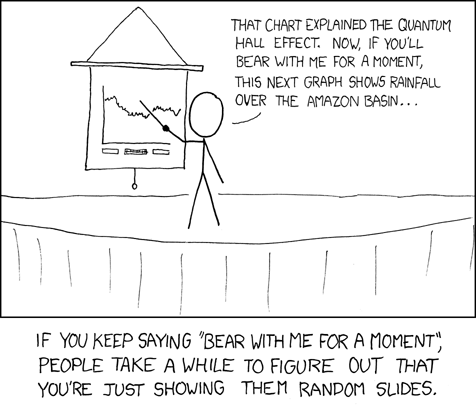
\includegraphics[height=2.5in]{slides.png}}
\end{frame}

\section{Math}

\begin{frame}{Math}
	You can use all math power of LaTeX easily doing something like this:
	\newline
	\centerline\
	$$\int_{a}^{b}( \alpha f(x) + \beta g(x))\,dx = \alpha \int_{a}^{b}f(x)\,dx + \beta \int_{a}^{b}g(x)\,dx$$
\end{frame}

\begin{frame}{}
		\LARGE{\centerline{Have a good luck with  \LaTeX\ Beamer!}}
\end{frame}

\end{document}